\let\negmedspace\undefined
\let\negthickspace\undefined
\documentclass[journal]{IEEEtran}
\usepackage[a5paper, margin=10mm, onecolumn]{geometry}
%\usepackage{lmodern} % Ensure lmodern is loaded for pdflatex
\usepackage{tfrupee} % Include tfrupee package

\setlength{\headheight}{1cm} % Set the height of the header box
\setlength{\headsep}{0mm}     % Set the distance between the header box and the top of the text

\usepackage{gvv-book}
\usepackage{gvv}
\usepackage{cite}
\usepackage{amsmath,amssymb,amsfonts,amsthm}
\usepackage{algorithmic}
\usepackage{graphicx}
\usepackage{textcomp}
\usepackage{xcolor}
\usepackage{txfonts}
\usepackage{listings}
\usepackage{enumitem}
\usepackage{mathtools}
\usepackage{gensymb}
\usepackage[breaklinks=true]{hyperref}
\usepackage{tkz-euclide} 
\usepackage{listings}
% \usepackage{gvv}                                        
\def\inputGnumericTable{}                                 
\usepackage[latin1]{inputenc}                                
\usepackage{color}                                            
\usepackage{array}                                            
\usepackage{longtable}                                       
\usepackage{calc}                                             
\usepackage{multirow}                                         
\usepackage{hhline}                                           
\usepackage{ifthen}                                           
\usepackage{lscape}
\usepackage{circuitikz}
\usepackage{comment}
\tikzstyle{block} = [rectangle, draw, fill=blue!20, 
    text width=4em, text centered, rounded corners, minimum height=3em]
\tikzstyle{sum} = [draw, fill=blue!10, circle, minimum size=1cm, node distance=1.5cm]
\tikzstyle{input} = [coordinate]
\tikzstyle{output} = [coordinate]


\begin{document}

\bibliographystyle{IEEEtran}
\vspace{3cm}

\title{9.4.39}
\author{EE25BTECH11026-Harsha}
 \maketitle
% \newpage
% \bigskip
{\let\newpage\relax\maketitle}

\renewcommand{\thefigure}{\theenumi}
\renewcommand{\thetable}{\theenumi}
\setlength{\intextsep}{10pt} % Space between text and floats


\numberwithin{equation}{enumi}
\numberwithin{figure}{enumi}
\renewcommand{\thetable}{\theenumi}

\textbf{Question}:\\
The difference of squares of two numbers is 180. The square of the smaller number is 8 times the larger number. Find the two numbers.\\
\solution \\
Let us solve the given question theoretically and then verify the solution computationally.\\
\\
Let x and y be the 2 numbers such that $x>y$.\\
The given equations are,
\begin{align}
    x^2-y^2=180 \label{eq:1}
\end{align}
\begin{align}
    y^2=8x \label{eq:2}
\end{align}
As the given equations are homogeneous, converting them into quadratic form,
\begin{align}
    \implies \vec{x}^{\top}\vec{V_1}\vec{x}+c=0 \label{eq:3}
\end{align}
where $\vec{x}^{\top}=\myvec{x&&y}$ and $\vec{V_1}=\myvec{1&&0\\0&&-1}$ and $c=-180$\\
And also,
\begin{align}
    \vec{x}^{\top}\vec{V_2}\vec{x}+2\vec{u}^{\top}\vec{x}=0 \label{eq:4}
\end{align}
where $\vec{x}^{\top}=\myvec{x&&y}^{\top}$, $\vec{V_2}=\myvec{0&&0\\0&&1}$ and $\vec{u}=\myvec{-4\\0}$.\\
To identify the intersection of conics, we can employ the approach of degenerating the conics.\\
\\
To work with degeneracy in matrix form we form the standard augmented $3 \times 3$ matrix for each conic:
\begin{align}
    \vec{M_i}=\myvec{\vec{V_i}&&\vec{u_i}\\\vec{u_i}^{\top}&&c_i} \label{eq:5}
\end{align}
From ~\eqref{eq:5},
\begin{align}
    \implies \vec{M_1}=\myvec{1&&0&&0\\0&&-1&&0\\0&&0&&-180} \quad 
    \vec{M_2}=\myvec{0&&0&&-4\\0&&1&&0\\-4&&0&&0}
\end{align}
\begin{align}
    \therefore \vec{x}^{\top}\brak{\vec{M_1+\lambda M_2}}\vec{x}=0
\end{align}
\newpage
\vspace*{0.25cm}
To degenerate the conic into a line, we can find the solutions of $\lambda$ when $\|\vec{M_1}+\lambda\vec{M_2}\|=0$ 
\begin{align}
    \therefore \|\vec{M_1}+\lambda\vec{M_2}\|=0 \label{eq:6}
\end{align}
\begin{align}
    \implies \brak{\lambda-1}\brak{4\lambda^2+45}=0
\end{align}
\begin{align}
    \therefore \lambda=1
\end{align}

Substituting $\lambda$ in ~\eqref{eq:6},
\begin{align}
    \implies \vec{x}^{\top}\brak{\vec{M_1}+\vec{M_2}}\vec{x}
\end{align}
\begin{align}
    \implies x^2-8x-180=0
\end{align}
\begin{align}
    \implies x=18,-10
\end{align}
for $x=-10$, there is no real solution of $y$ in ~\eqref{eq:2},
\begin{align}
    \implies y=\pm 12
\end{align}
\begin{align}
    \therefore \text{The two numbers are }\brak{18,12}\, and\, \brak{18,-12}
\end{align}
From the figure, it is clearly verified that the theoretical solution matches with the computational solution.\\
\begin{figure}[H]
    \centering
    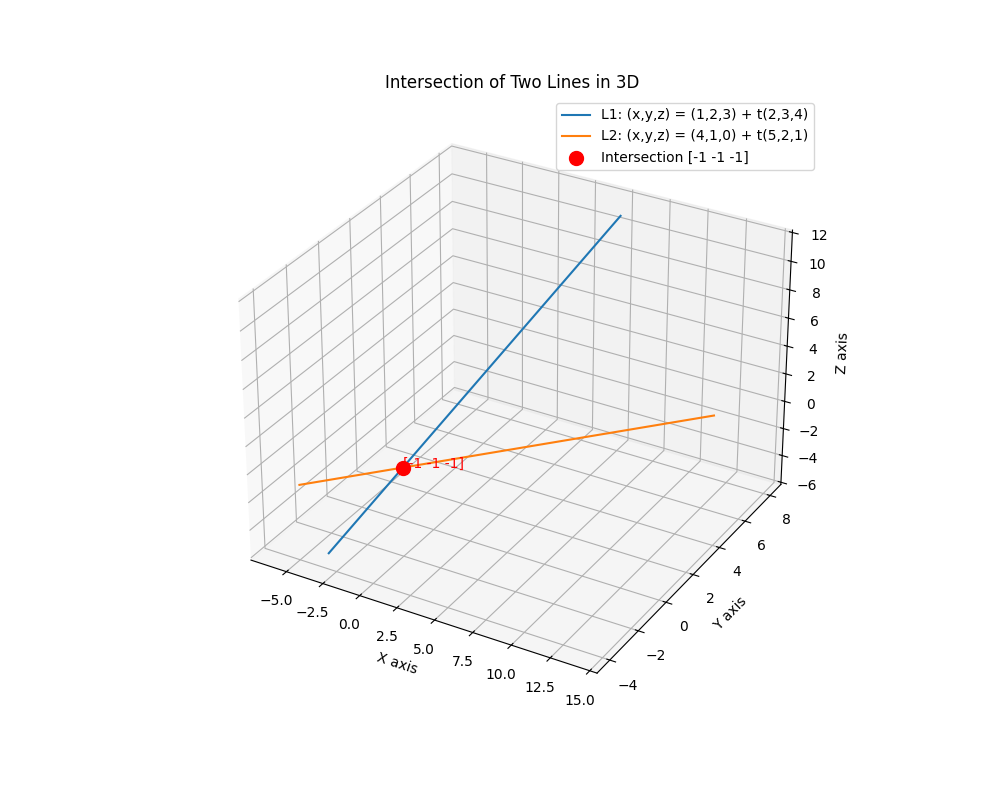
\includegraphics[width=0.6\columnwidth]{figs/Figure_1.png}
    \label{fig:1}
\end{figure}


\end{document}
